%Autor: Simon Walker
%Version: 1.0
%Datum: 10.11.2019

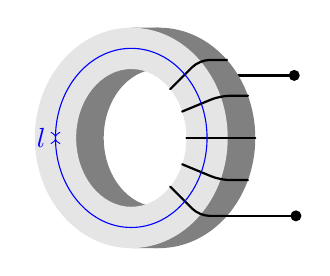
\begin{tikzpicture}[xscale=0.7, yscale=0.7, line cap=round, line join=round]
%\draw[help lines] (-2,-2) grid (3,2);
\draw [thick] (-45:1.75 and 2) -- ++(1.75,0) coordinate (a);
\draw [thick] (45:1 and 1.25)++(0,0.25) -- ++(2.25,0) coordinate (b);
\fill (a) circle [radius=.1] (b) circle [radius=.1];

\fill [gray, even odd rule] (0.5,0) 
  ellipse [x radius=1.75, y radius=2] ellipse [x radius=1, y radius=1.25];
\fill [gray] (0,2) rectangle ++(0.5, -0.25) (0,-2) rectangle ++(0.5, 0.25);
\fill [gray!20, even odd rule] 
  ellipse [x radius=1.75, y radius=2] ellipse [x radius=1, y radius=1.25];
\foreach \i in {-45,-22.5,...,45}
  \draw [thick, rounded corners=0.125cm] 
    (\i:1 and 1.25) -- (\i:1.75 and 2) -- +(0.5,0);
 
\draw [blue] ellipse [x radius=1.375, y radius=1.625];
\draw [blue, >-<] (-1.375, -0.11) -- (-1.375, 0.11);
\node [blue, left] at (-1.375, 0) {$l$};
 
\end{tikzpicture}
